\documentclass[aspectratio=169,10pt]{beamer}

\usetheme{Madrid}
\usecolortheme{whale}

\usepackage[spanish,es-tabla]{babel}
\usepackage{graphicx}
\usepackage{booktabs}
\usepackage{xcolor}
\usepackage{amsmath}
% amssymb eliminado: boldsymbol carga nullfont en contextos beamer
\usepackage{tikz}
\usetikzlibrary{positioning}
\usepackage{array}

\graphicspath{
  {../../outputs/figures/step6/}
  {../../outputs/figures/step7/}
  {../../outputs/figures/step8/}
}

\definecolor{bdrplus}{RGB}{31,119,180}
\definecolor{bdrminus}{RGB}{214,39,40}
\definecolor{controls}{RGB}{44,160,44}
\definecolor{subtletext}{RGB}{100,100,100}
\definecolor{darkblue}{RGB}{0,51,102}

\setbeamertemplate{navigation symbols}{}
\setbeamertemplate{footline}{
  \leavevmode\hbox{%
    \begin{beamercolorbox}[wd=.33\paperwidth,ht=2.25ex,dp=1ex,center]{author in head/foot}
      \usebeamerfont{author in head/foot}\insertshortauthor
    \end{beamercolorbox}%
    \begin{beamercolorbox}[wd=.34\paperwidth,ht=2.25ex,dp=1ex,center]{title in head/foot}
      \usebeamerfont{title in head/foot}\insertshorttitle
    \end{beamercolorbox}%
    \begin{beamercolorbox}[wd=.33\paperwidth,ht=2.25ex,dp=1ex,right]{date in head/foot}
      \usebeamerfont{date in head/foot}\insertframenumber{}/\inserttotalframenumber\hspace*{2ex}
    \end{beamercolorbox}}%
}

\title[CAS como biomarcador BD]{%
  Evaluación de la Respuesta Broncodilatadora\\
  mediante Análisis de Sonidos Respiratorios}
\author[Oliva \textperiodcentered{} Vila \textperiodcentered{} Font \textperiodcentered{} Cardona \textperiodcentered{} Manzano]{%
  \footnotesize
  Lorenzo Oliva \enspace\textperiodcentered\enspace
  Martina Vila López \enspace\textperiodcentered\enspace
  Adrià Font Plana \\
  Antoni Cardona Riera \enspace\textperiodcentered\enspace
  Gabriel Manzano Reche}
\institute[UPC]{Digital Biomarkers}
\date{Junio 2026}

% ════════════════════════════════════════════════════════════════════════════
\begin{document}

% ── SLIDE 1: Título ──────────────────────────────────────────────────────────
\begin{frame}
  \titlepage
\end{frame}

% ── SLIDE 2: Motivación y objetivo ──────────────────────────────────────────
\begin{frame}{Motivación y Objetivo}
  \begin{columns}
    \column{0.52\textwidth}
      \begin{block}{Contexto clínico}
        \begin{itemize}
          \item \textbf{Asma}: obstrucción bronquial reversible
          \item \textbf{Broncodilatador (BD)}: relaja la musculatura
          \item No todos responden igual: \textbf{BDR+} vs \textbf{BDR--}
          \item Gold standard: \alert{espirometría} (flujo de aire)
        \end{itemize}
      \end{block}
      \begin{block}{Nuestra propuesta}
        \begin{itemize}
          \item CAS (\textit{Crackle-like Adventitious Sounds}): sonidos anómalos en señal respiratoria
          \item Hipótesis: variación CAS pre/post-BD como biomarcador digital
        \end{itemize}
      \end{block}
    \column{0.44\textwidth}
      \begin{block}{Objetivo}
        Clasificar automáticamente CAS y usar su variación pre/post-BD como \textbf{biomarcador digital} de respuesta broncodilatadora.
      \end{block}
      \begin{alertblock}{Ventaja}
        Análisis de audio pasivo y no invasivo
      \end{alertblock}
  \end{columns}
\end{frame}

% ── SLIDE 3: Dataset ────────────────────────────────────────────────────────
\begin{frame}{Dataset Experimental}
  \begin{columns}
    \column{0.48\textwidth}
      \begin{block}{Participantes}
        \centering\small
        \begin{tabular}{lc}
          \toprule
          \textbf{Grupo} & \textbf{n} \\
          \midrule
          BDR+ & 9 \\
          BDR-- & 14 \\
          Controles & 5 \\
          \midrule
          \textbf{Total} & \textbf{28} \\
          \bottomrule
        \end{tabular}
      \end{block}
      \begin{block}{Protocolo}
        \begin{itemize}\small
          \item 2 canales: inferior ch1 + superior ch2
          \item 6 maniobras: 3 pre-BD + 3 post-BD
          \item Frecuencia de muestreo: 12\,500\,Hz
        \end{itemize}
      \end{block}
    \column{0.48\textwidth}
      \begin{block}{Señales generadas}
        \centering\small
        \begin{tabular}{lc}
          \toprule
          \textbf{Concepto} & \textbf{Valor} \\
          \midrule
          Total segmentos & 14\,900 \\
          Etiquetados & 1\,923 \\
          \quad CAS & 590 (30.7\,\%) \\
          \quad NO CAS & 1\,333 (69.3\,\%) \\
          \bottomrule
        \end{tabular}
      \end{block}
      \begin{alertblock}{Desequilibrio de clases}
        \centering\small
        Ratio 1:2.3 (CAS:NO\,CAS)
      \end{alertblock}
  \end{columns}
\end{frame}

% ── SLIDE 4: Pipeline ───────────────────────────────────────────────────────
\begin{frame}{Pipeline de Procesado}
  \centering
  \begin{tikzpicture}[
    box/.style={draw, rounded corners=4pt, fill=darkblue!15,
                text width=2.55cm, align=center, minimum height=1.0cm, font=\small},
    arr/.style={->, thick, darkblue},
    node distance=0.45cm
  ]
    \node[box] (A) {\textbf{Lectura}\\\small\texttt{read\_signals()}};
    \node[box, right=of A] (B) {\textbf{Preprocesado}\\\small 3 pasos};
    \node[box, right=of B] (C) {\textbf{Segmentación}\\\small marcas tPX};
    \node[box, right=of C] (D) {\textbf{Features}\\\small 15 features};
    \node[box, right=of D] (E) {\textbf{Clasificador}\\RF / SVM\\\small LOSO};
    \draw[arr] (A)--(B); \draw[arr] (B)--(C);
    \draw[arr] (C)--(D); \draw[arr] (D)--(E);
  \end{tikzpicture}

  \begin{columns}
    \column{0.32\textwidth}
      \begin{block}{\small Preprocesado}
        \begin{enumerate}\footnotesize
          \item Remuestreo $12\,500 \to 4\,000$\,Hz
          \item Butterworth ord.\,8 (70--1900\,Hz)
          \item Filtro comb notch 50\,Hz + armónicos
        \end{enumerate}
      \end{block}
    \column{0.32\textwidth}
      \begin{block}{\small Segmentación}
        \begin{itemize}\footnotesize
          \item Marcas tPX.mat: ciclos respiratorios
          \item Resultado: insp. + esp. por canal
        \end{itemize}
      \end{block}
    \column{0.32\textwidth}
      \begin{block}{\small 4 vectores metadatos}
        \begin{itemize}\footnotesize
          \item Sujeto (1--28)
          \item Pre/post-BD (1/2)
          \item Canal (1/2)
          \item Fase insp./esp. (1/2)
        \end{itemize}
      \end{block}
  \end{columns}
\end{frame}

% ── SLIDE 5: LOSO ───────────────────────────────────────────────────────────
\begin{frame}{Estrategia de Clasificación: LOSO}
  \begin{columns}
    \column{0.48\textwidth}
      \begin{block}{¿Por qué Leave-One-Subject-Out?}
        \begin{itemize}
          \item 1\,923 señales de \textbf{18 sujetos} agrupados
          \item Split aleatorio $\Rightarrow$ \alert{data leakage}
          \item LOSO: modelo nunca ve al sujeto de test
        \end{itemize}
      \end{block}
      \begin{exampleblock}{17 folds (P8 excluido: 3 CAS)}
        \footnotesize
        Fold 1: \textbf{[TEST: P1]} [TRAIN: P2\ldots P17]\\
        Fold 2: \textbf{[TEST: P2]} [TRAIN: P1,P3\ldots P17]\\
        \hspace{1em}\vdots\\
        Fold 17: \textbf{[TEST: P23]} [TRAIN: resto]
      \end{exampleblock}
    \column{0.48\textwidth}
      \begin{block}{Pipeline}
        \centering\small
        \begin{tikzpicture}[
          pipenode/.style={draw, fill=bdrplus!15, rounded corners=3pt,
                           text width=3.5cm, align=center,
                           minimum height=0.65cm, font=\small},
          arr/.style={->, thick}]
          \node[pipenode] (s) {StandardScaler};
          \node[pipenode, below=0.25cm of s] (k) {SelectKBest ($k=10$)};
          \node[pipenode, below=0.25cm of k] (c) {SVM / RF / XGB / Ensemble};
          \draw[arr] (s)--(k); \draw[arr] (k)--(c);
        \end{tikzpicture}
      \end{block}
      \begin{block}{15 features acústicas}
        \footnotesize RMS, duración, ZCR, kurtosis, skewness, TKEO, frec.\ dominante, frec.\ media, 4$\times$ band power, entropía espectral, razón armónica, sample entropy
      \end{block}
  \end{columns}
\end{frame}

% ── SLIDE 6: Resultados LOSO ────────────────────────────────────────────────
\begin{frame}{Resultados LOSO --- Comparativa de Modelos}
  \begin{columns}
    \column{0.55\textwidth}
      \begin{block}{}
        \centering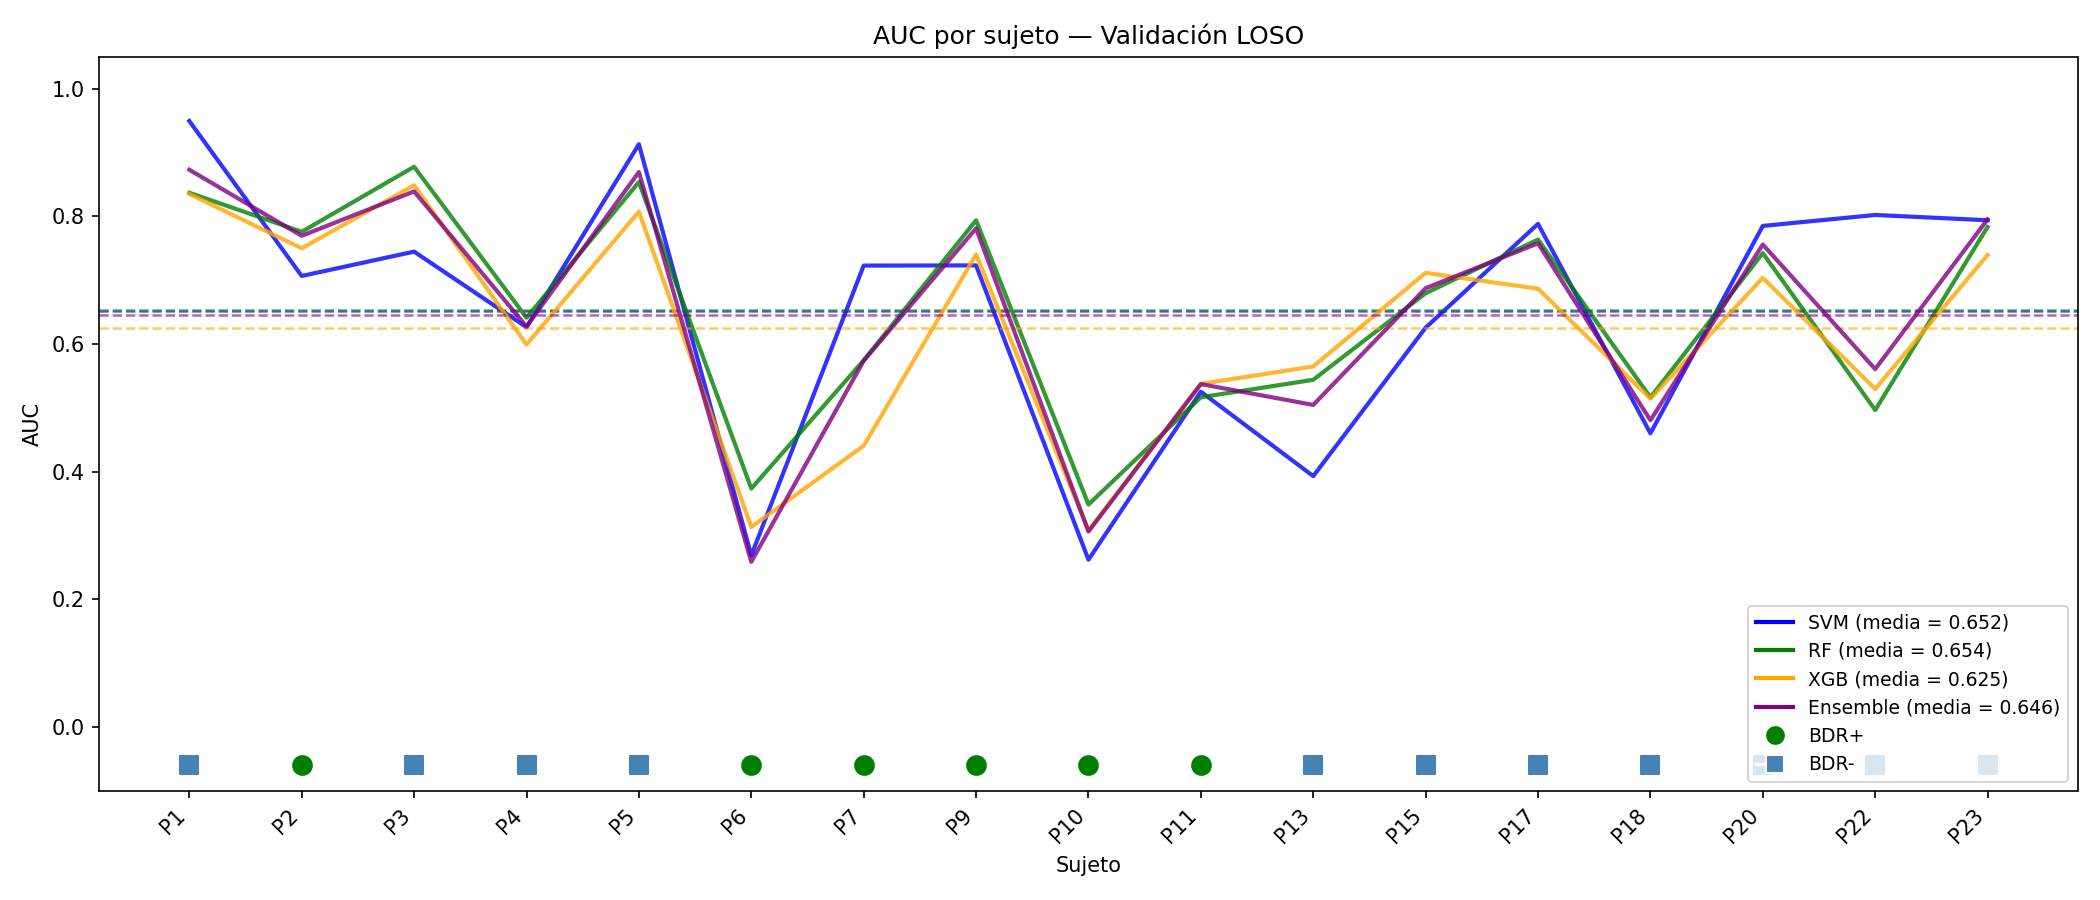
\includegraphics[width=0.97\linewidth]{fig3_loso_auc_per_fold.png}
      \end{block}
    \column{0.42\textwidth}
      \begin{block}{Métricas medias (17 folds)}
        \centering\footnotesize
        \begin{tabular}{lccc}
          \toprule
          \textbf{Modelo} & \textbf{AUC} & \textbf{Sens.} & \textbf{Spec.} \\
          \midrule
          SVM        & 0.652 & 0.500 & 0.750 \\
          \textbf{RF}& \textbf{0.654} & 0.335 & 0.886 \\
          XGB        & 0.625 & 0.422 & 0.775 \\
          Ensemble   & 0.646 & 0.385 & 0.852 \\
          \bottomrule
        \end{tabular}
      \end{block}
      \begin{alertblock}{Interpretación}
        \footnotesize Alta varianza ($\pm$0.20) por heterogeneidad inter-sujeto. Rango: 0.26--0.95
      \end{alertblock}
      \begin{exampleblock}{\small Modelo final}
        \centering\small\textbf{RF} (mejor AUC LOSO)
      \end{exampleblock}
  \end{columns}
\end{frame}

% ── SLIDE 7: Modelo final ────────────────────────────────────────────────────
\begin{frame}{Modelo Final: Inferencia sobre 14\,900 Señales}
  \begin{columns}
    \column{0.46\textwidth}
      \begin{block}{Clasificación completa}
        \begin{itemize}
          \item RF reentrenado con \textbf{1\,923} señales etiquetadas
          \item Aplicado a \textbf{14\,900} señales totales
          \item Resultado: \textbf{2\,698 CAS detectados} (18.1\,\%)
        \end{itemize}
      \end{block}
      \begin{exampleblock}{Siguiente paso}
        \small Calcular $\Delta$CAS por sujeto, canal y fase respiratoria
      \end{exampleblock}
    \column{0.50\textwidth}
      \begin{block}{}
        \centering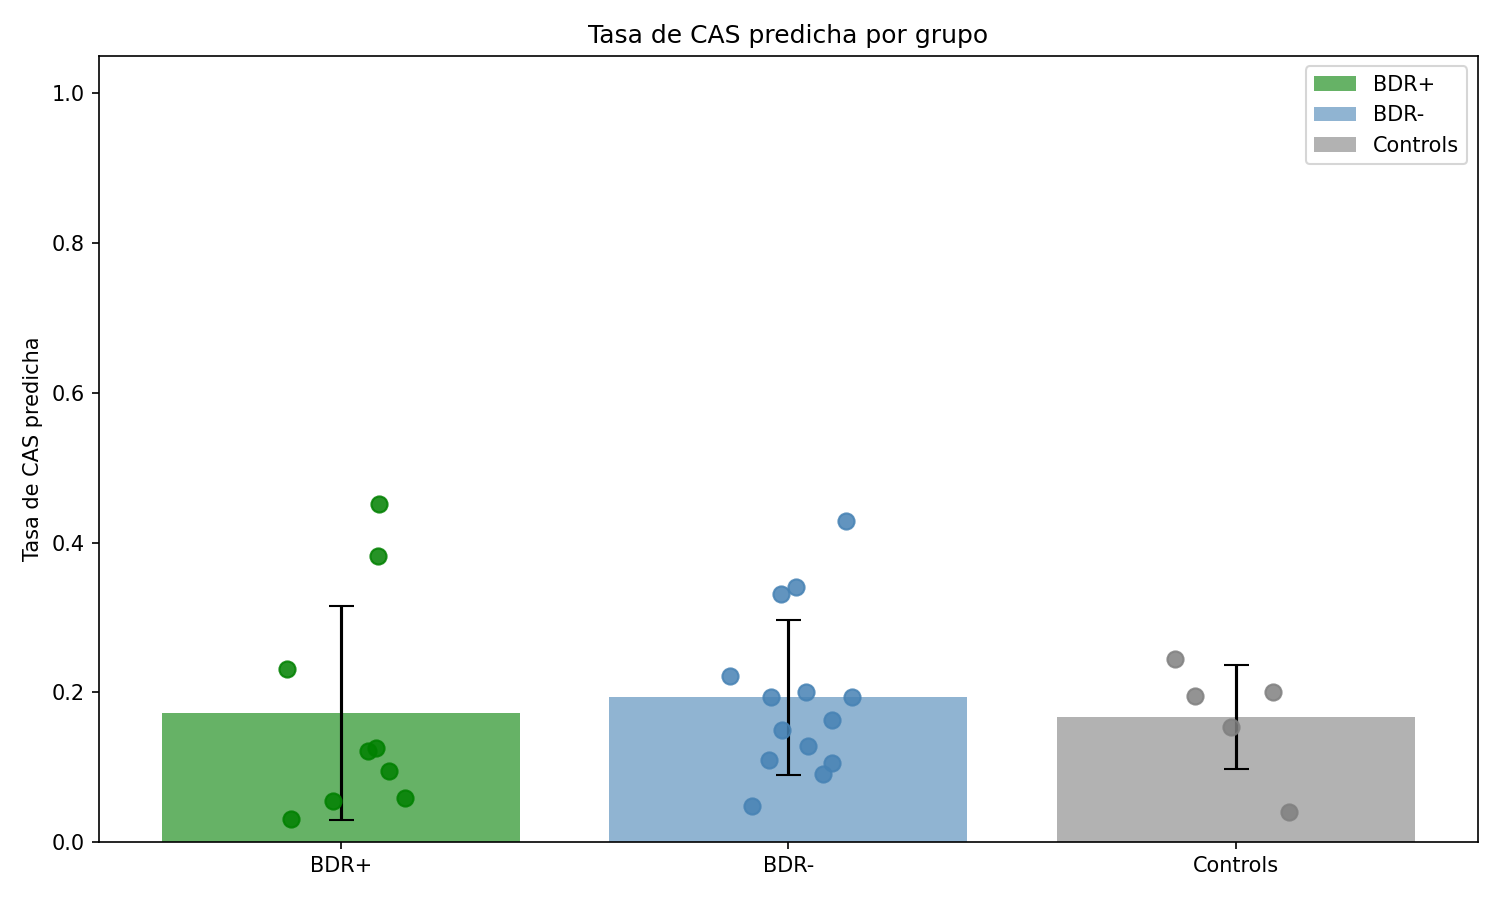
\includegraphics[width=0.97\linewidth]{fig5_cas_rate_by_group.png}
      \end{block}
  \end{columns}
\end{frame}

% ── SLIDE 8: Biomarcador ΔCAS ────────────────────────────────────────────────
\begin{frame}{Biomarcador Digital: $\Delta$CAS}
  \begin{columns}
    \column{0.50\textwidth}
      \begin{block}{Definición}
        \begin{tabular}{c}
          $\displaystyle\Delta\text{CAS} = 100 \times \dfrac{N_{\text{CAS}}^{\text{pre}} - N_{\text{CAS}}^{\text{post}}}{N_{\text{CAS}}^{\text{pre}}}$
        \end{tabular}
      \end{block}
      \begin{block}{Interpretación}
        \begin{itemize}
          \item \textcolor{controls}{$\Delta$CAS $> 0$}: reducción $\Rightarrow$ BDR+
          \item \textcolor{bdrminus}{$\Delta$CAS $< 0$}: aumento $\Rightarrow$ sin respuesta
        \end{itemize}
      \end{block}
      \begin{alertblock}{Limitación}
        \small $N_\text{CAS}^\text{pre}$ bajo $\Rightarrow$ valores extremos
      \end{alertblock}
    \column{0.46\textwidth}
      \begin{block}{Ejemplos individuales}
        \centering\small
        \begin{tabular}{lcc}
          \toprule
          \textbf{Sujeto} & \textbf{Grupo} & \textbf{$\Delta$CAS} \\
          \midrule
          P9  & \textcolor{bdrplus}{BDR+}  & \textcolor{controls}{+65\,\%} \\
          P2  & \textcolor{bdrplus}{BDR+}  & \textcolor{controls}{+35\,\%} \\
          P11 & \textcolor{bdrplus}{BDR+}  & \textcolor{controls}{+20\,\%} \\
          \midrule
          P13 & \textcolor{bdrminus}{BDR--} & \textcolor{bdrminus}{$-$103\,\%} \\
          P18 & \textcolor{bdrminus}{BDR--} & \textcolor{bdrminus}{$-$122\,\%} \\
          \bottomrule
        \end{tabular}
      \end{block}
  \end{columns}
\end{frame}

% ── SLIDE 9: Resultados ΔCAS por grupo ──────────────────────────────────────
\begin{frame}{Resultados $\Delta$CAS por Grupo Clínico}
  \begin{columns}
    \column{0.50\textwidth}
      \begin{block}{}
        \centering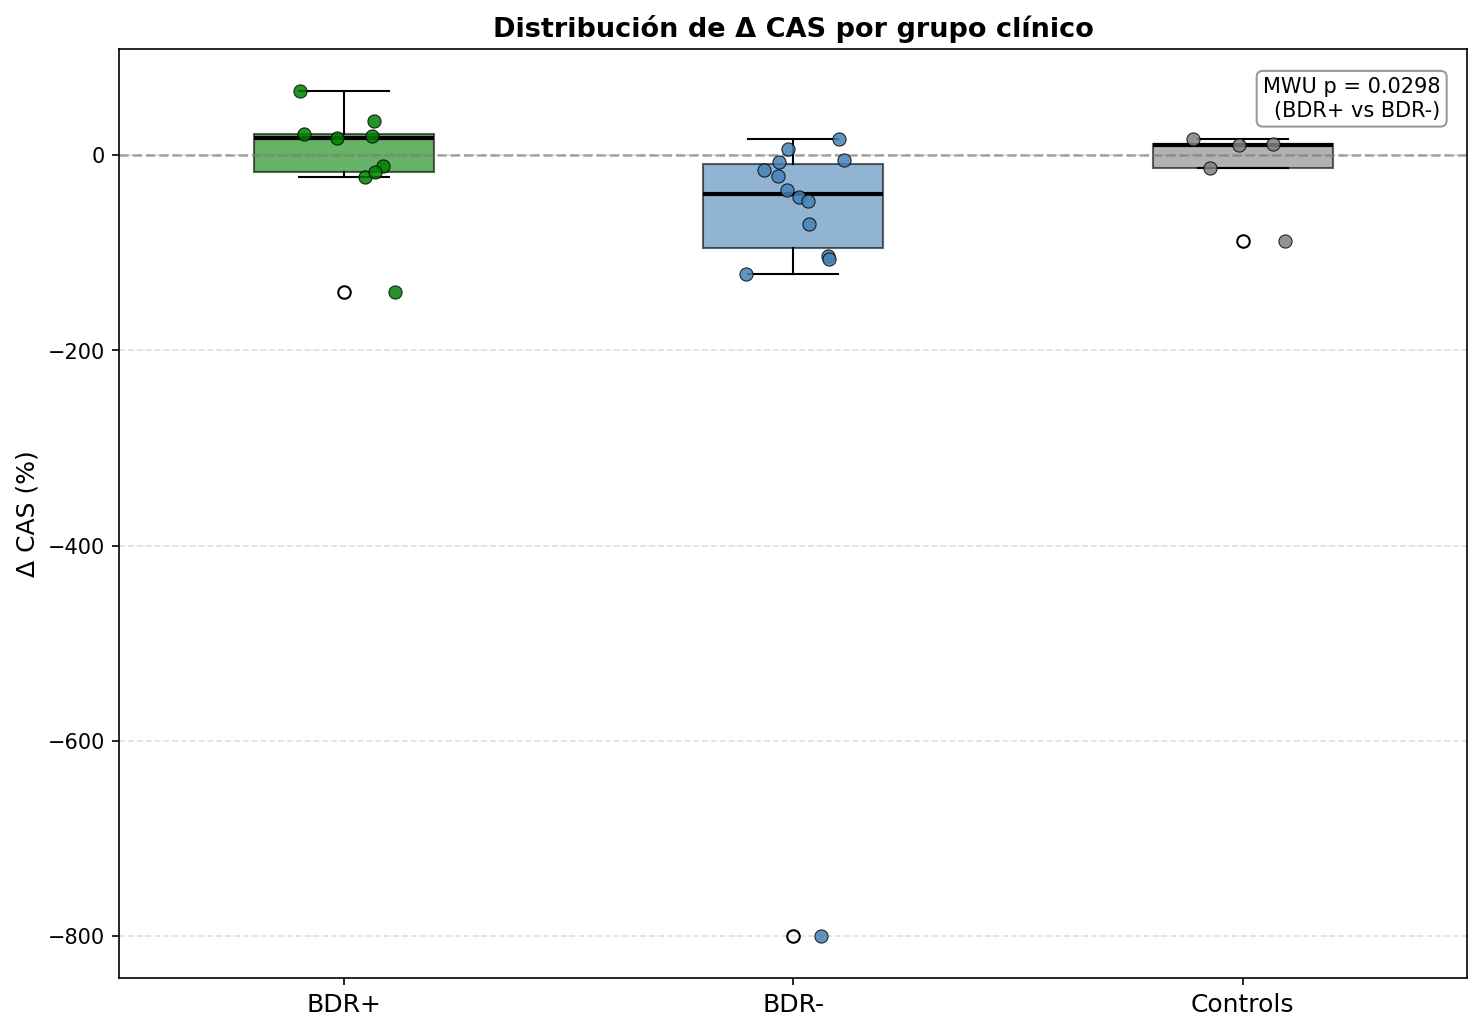
\includegraphics[width=0.97\linewidth]{fig3_boxplot_delta_cas.png}
      \end{block}
    \column{0.47\textwidth}
      \begin{block}{$\Delta$CAS por grupo}
        \centering\small
        \begin{tabular}{lccc}
          \toprule
          \textbf{Grupo} & \textbf{n} & \textbf{$\Delta$CAS} & \textbf{pre} \\
          \midrule
          \textcolor{bdrplus}{BDR+}  & 9  & $-3.4\pm58$   & 18.9\,\% \\
          \textcolor{bdrminus}{BDR--} & 14 & $-97\pm207$   & 16.3\,\% \\
          \textcolor{controls}{Ctrl} & 5  & $-12\pm44$    & 17.0\,\% \\
          \bottomrule
        \end{tabular}
      \end{block}
      \begin{exampleblock}{\textbf{Tests estadísticos}}
        \small\begin{tabular}{ll}
          MWU (BDR+ vs BDR--): & {\large\textbf{p=0.030}} \textcolor{controls}{$\checkmark$} \\
          KW (3 grupos):        & {\large\textbf{p=0.041}} \textcolor{controls}{$\checkmark$} \\
        \end{tabular}
      \end{exampleblock}
  \end{columns}
\end{frame}

% ── SLIDE 10: ΔCAS por canal y fase ─────────────────────────────────────────
\begin{frame}{$\Delta$CAS por Canal y Fase Respiratoria}
  \begin{columns}
    \column{0.50\textwidth}
      \begin{block}{}
        \centering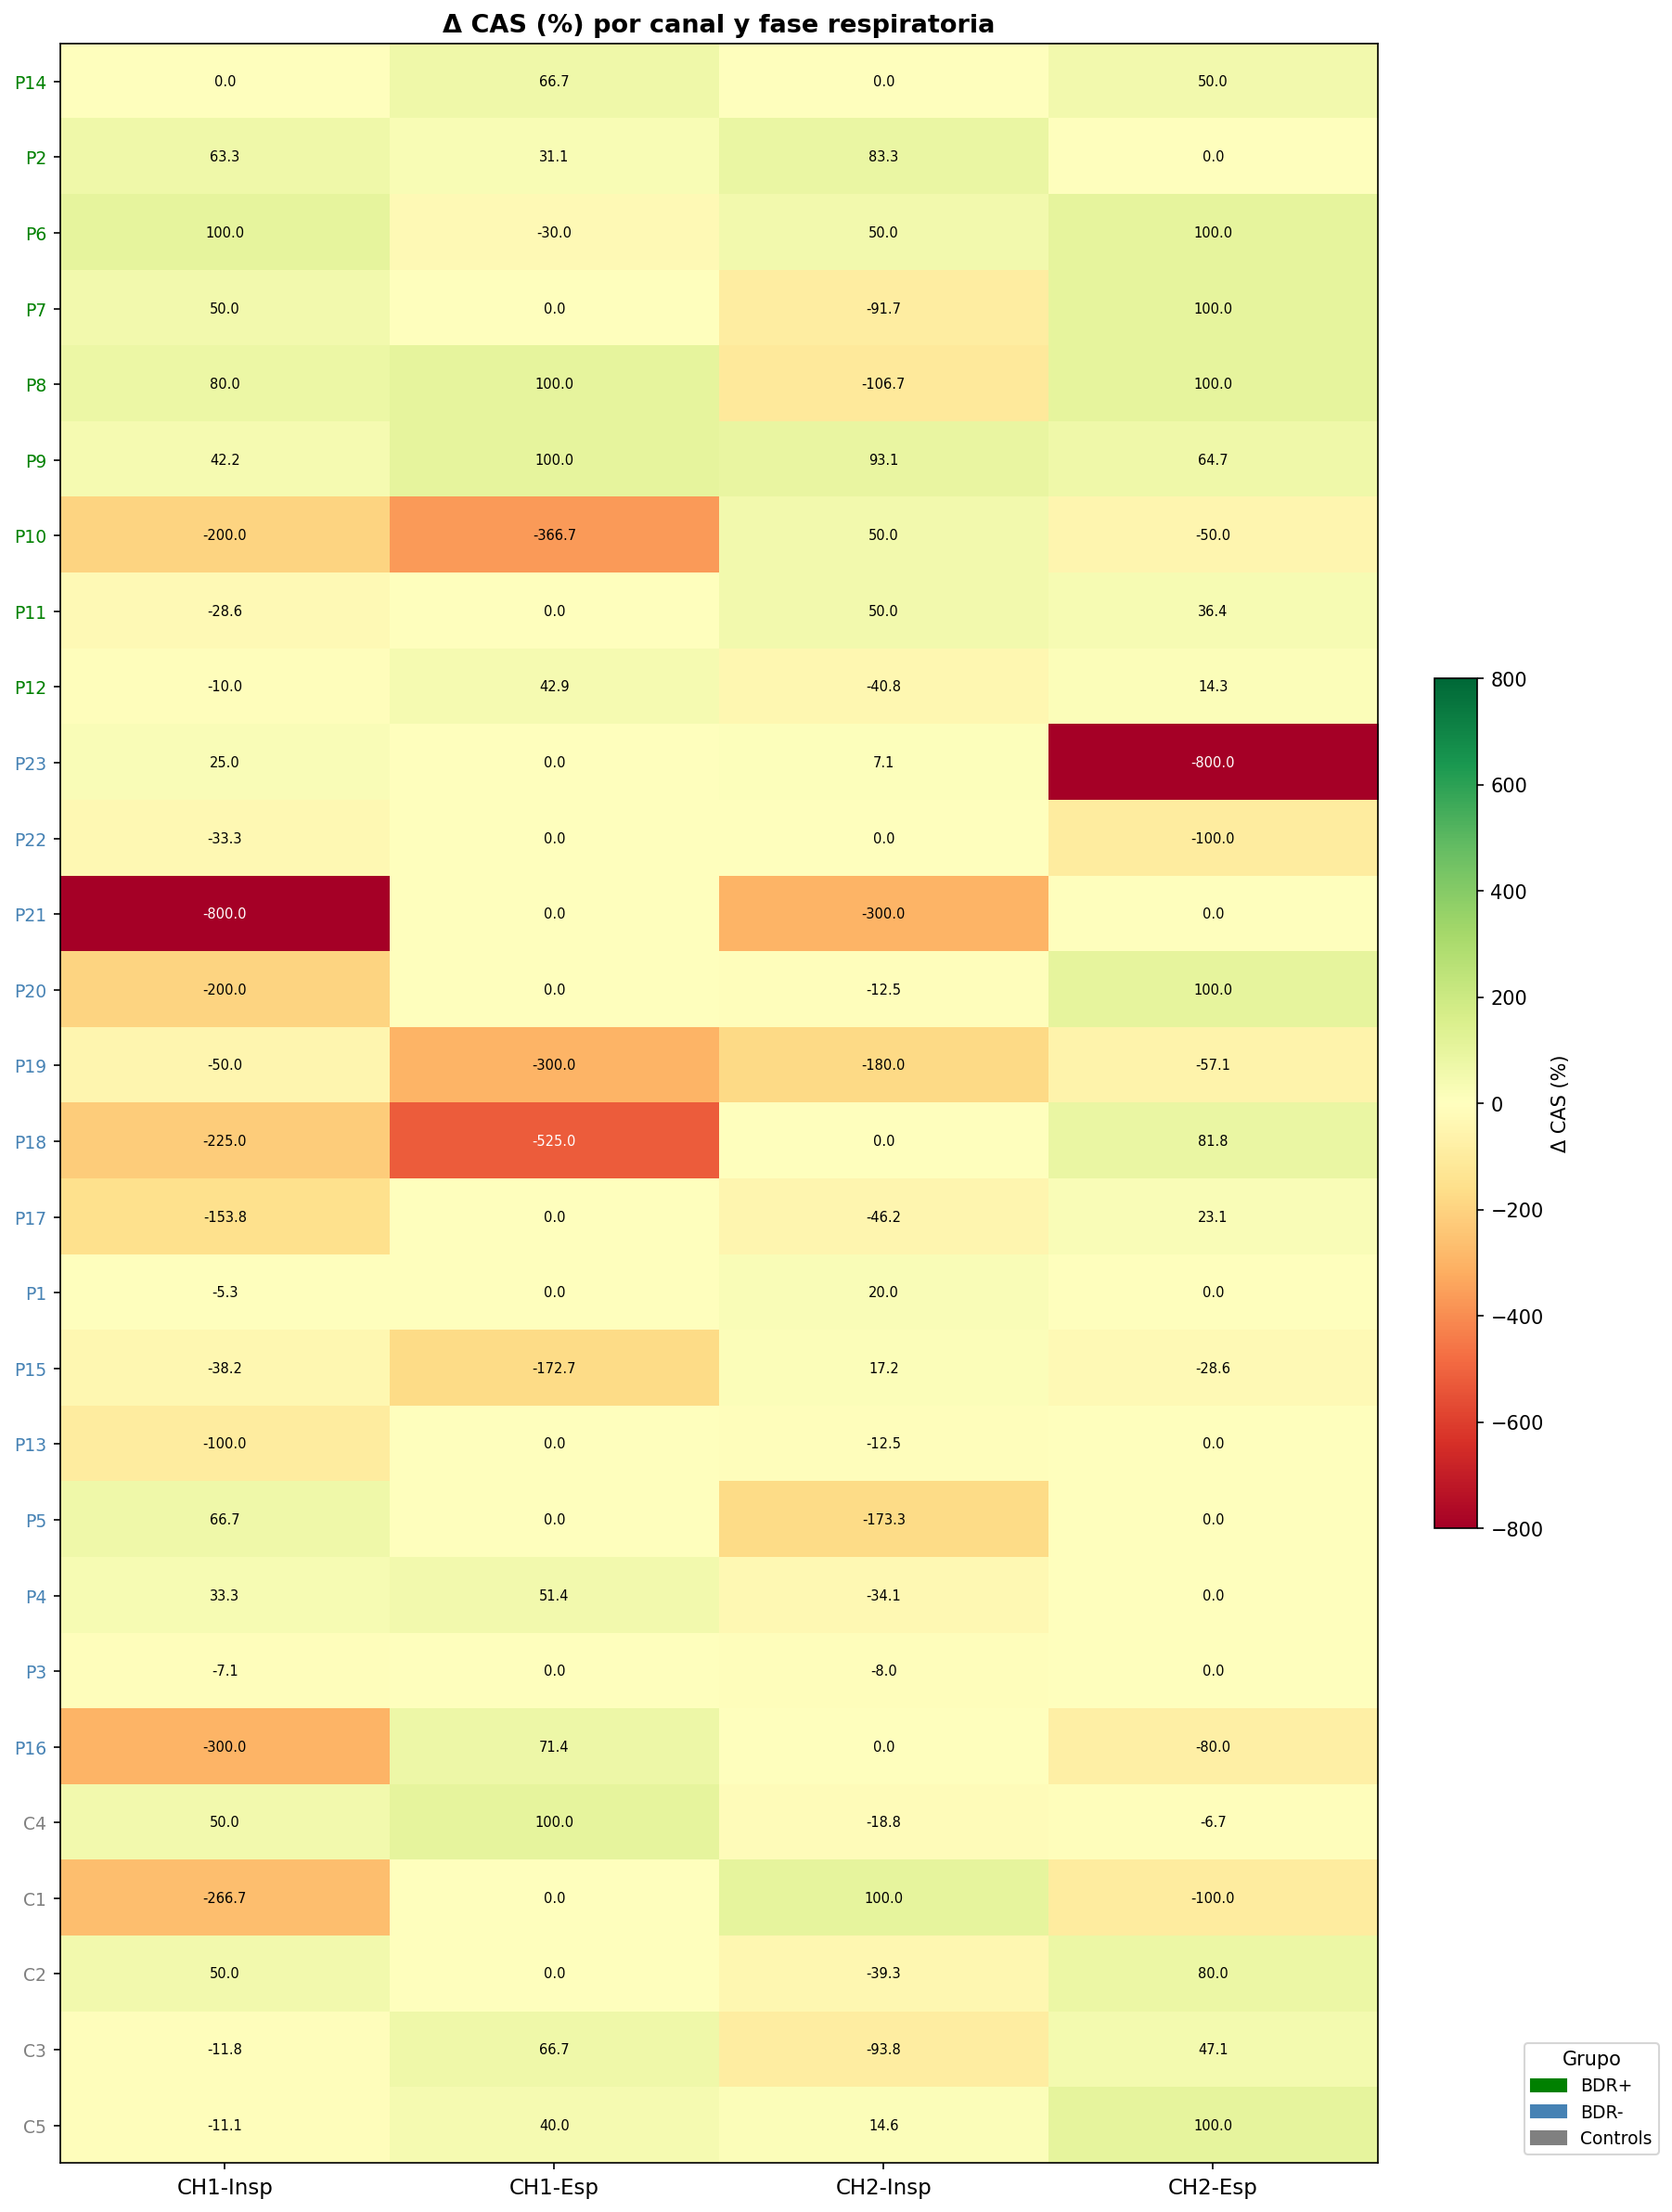
\includegraphics[width=0.97\linewidth]{fig4_heatmap_delta_cas.png}
      \end{block}
    \column{0.47\textwidth}
      \begin{block}{Por fase (\%)}
        \centering\small
        \begin{tabular}{lcc}
          \toprule
          \textbf{Grupo} & \textbf{Insp.} & \textbf{Esp.} \\
          \midrule
          \textcolor{bdrplus}{BDR+}  & $+12\pm45$ & $+22\pm84$ \\
          \textcolor{bdrminus}{BDR--} & $-114\pm189$ & $-86\pm236$ \\
          \textcolor{controls}{Ctrl} & $-21\pm43$   & $+22\pm73$ \\
          \bottomrule
        \end{tabular}
      \end{block}
      \begin{block}{Por canal (\%)}
        \centering\small
        \begin{tabular}{lcc}
          \toprule
          \textbf{Grupo} & \textbf{ch1} & \textbf{ch2} \\
          \midrule
          \textcolor{bdrplus}{BDR+}  & $-11\pm122$ & $+7\pm55$ \\
          \textcolor{bdrminus}{BDR--} & $-127\pm253$ & $-67\pm143$ \\
          \textcolor{controls}{Ctrl} & $-31\pm132$ & $-2\pm23$ \\
          \bottomrule
        \end{tabular}
      \end{block}
      \begin{exampleblock}{}
        \footnotesize\textcolor{darkblue}{\textbf{ch2 e inspiración}: condiciones más discriminativas}
      \end{exampleblock}
  \end{columns}
\end{frame}

% ── SLIDE 11: Deep Learning ──────────────────────────────────────────────────
\begin{frame}{Comparativa: Deep Learning vs.\ Features Manuales}
  \begin{columns}
    \column{0.48\textwidth}
      \begin{block}{}
        \centering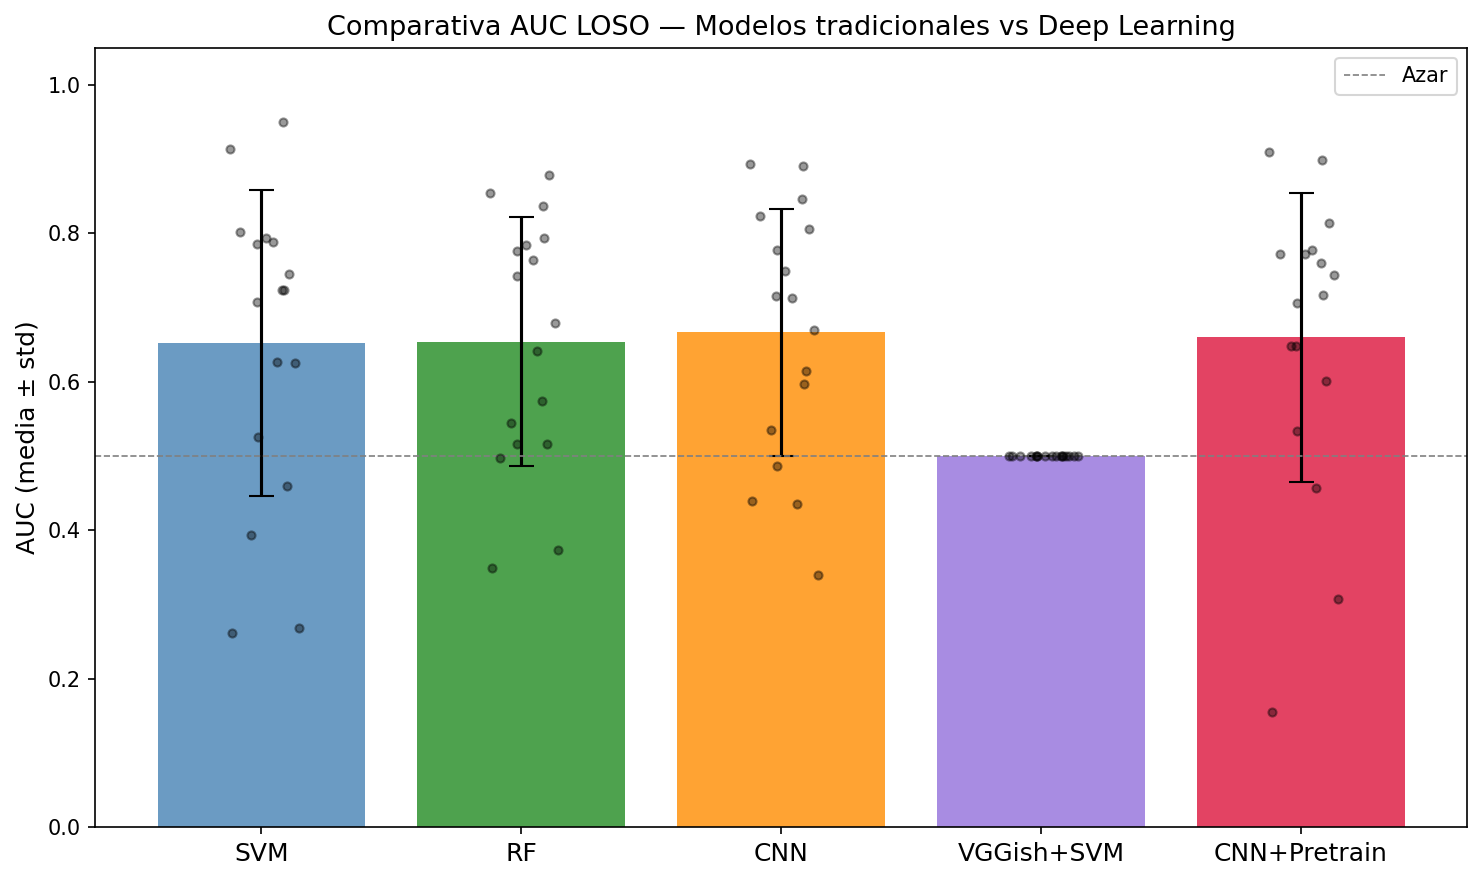
\includegraphics[width=0.97\linewidth]{fig2_auc_comparison.png}
      \end{block}
    \column{0.49\textwidth}
      \begin{block}{Resultados LOSO}
        \centering\footnotesize
        \begin{tabular}{lcc}
          \toprule
          \textbf{Modelo} & \textbf{AUC} & \textbf{Sens.} \\
          \midrule
          SVM baseline & 0.652 & 0.500 \\
          RF baseline  & 0.654 & 0.335 \\
          CNN scratch  & 0.666 & 0.524 \\
          CNN+Pretrain & 0.660 & \textbf{0.623} \\
          VGGish+SVM   & 0.500 & --- \\
          \bottomrule
        \end{tabular}
      \end{block}
      \begin{block}{Conclusiones DL}
        \begin{itemize}\footnotesize
          \item CNN $\approx$ RF en AUC con n=1\,923
          \item Pretrain semisupervisado mejora sensitivity ($0.52 \to 0.62$)
          \item VGGish: mismatch de dominio (16\,kHz genérico)
        \end{itemize}
      \end{block}
  \end{columns}
\end{frame}

% ── SLIDE 12: Limitaciones ───────────────────────────────────────────────────
\begin{frame}{Limitaciones del Estudio}
  \begin{alertblock}{Técnicas}
    \begin{itemize}\small
      \item n=1\,923 etiquetadas $\Rightarrow$ varianza LOSO alta ($\pm$0.20)
      \item Etiquetas en 18/23 pacientes; sin controles etiquetados
      \item $\Delta$CAS inestable con pocos CAS pre-BD
      \item Clasificador validado principalmente en ch1
    \end{itemize}
  \end{alertblock}
  \begin{alertblock}{Clínicas}
    \begin{itemize}\small
      \item n=23 pacientes: potencia estadística limitada
      \item Sin validación vs espirometría (gold standard)
      \item Alta variabilidad fisiológica inter-sujeto
      \item Solo 6 maniobras; sin reproducibilidad inter-sesión
    \end{itemize}
  \end{alertblock}
\end{frame}

% ── SLIDE 13: Conclusiones ───────────────────────────────────────────────────
\begin{frame}{Conclusiones}
  \begin{enumerate}\setlength{\itemsep}{9pt}
    \item \textbf{Pipeline completo:} 14\,900 señales procesadas (lectura $\to$ preprocesado $\to$ segmentación $\to$ features $\to$ clasificación)
    \item \textbf{Rendimiento:} RF con AUC\,=\,0.654\,$\pm$\,0.167 en validación LOSO por sujeto
    \item \textcolor{darkblue}{\textbf{Resultado principal:}} $\Delta$CAS discrimina BDR+ de BDR-- (\textbf{p\,=\,0.030}), tendencia consistente en ch2 e inspiración
    \item \textbf{Deep Learning:} CNN comparable a RF; preentrenamiento semisupervisado mejora sensitivity ($0.52 \to 0.62$)
    \item \textbf{Limitación principal:} n insuficiente para DL robusto y conclusiones clínicas definitivas
  \end{enumerate}
\end{frame}

% ── SLIDE 14: Preguntas ──────────────────────────────────────────────────────
\begin{frame}{¿Preguntas?}
  \begin{block}{}
    \centering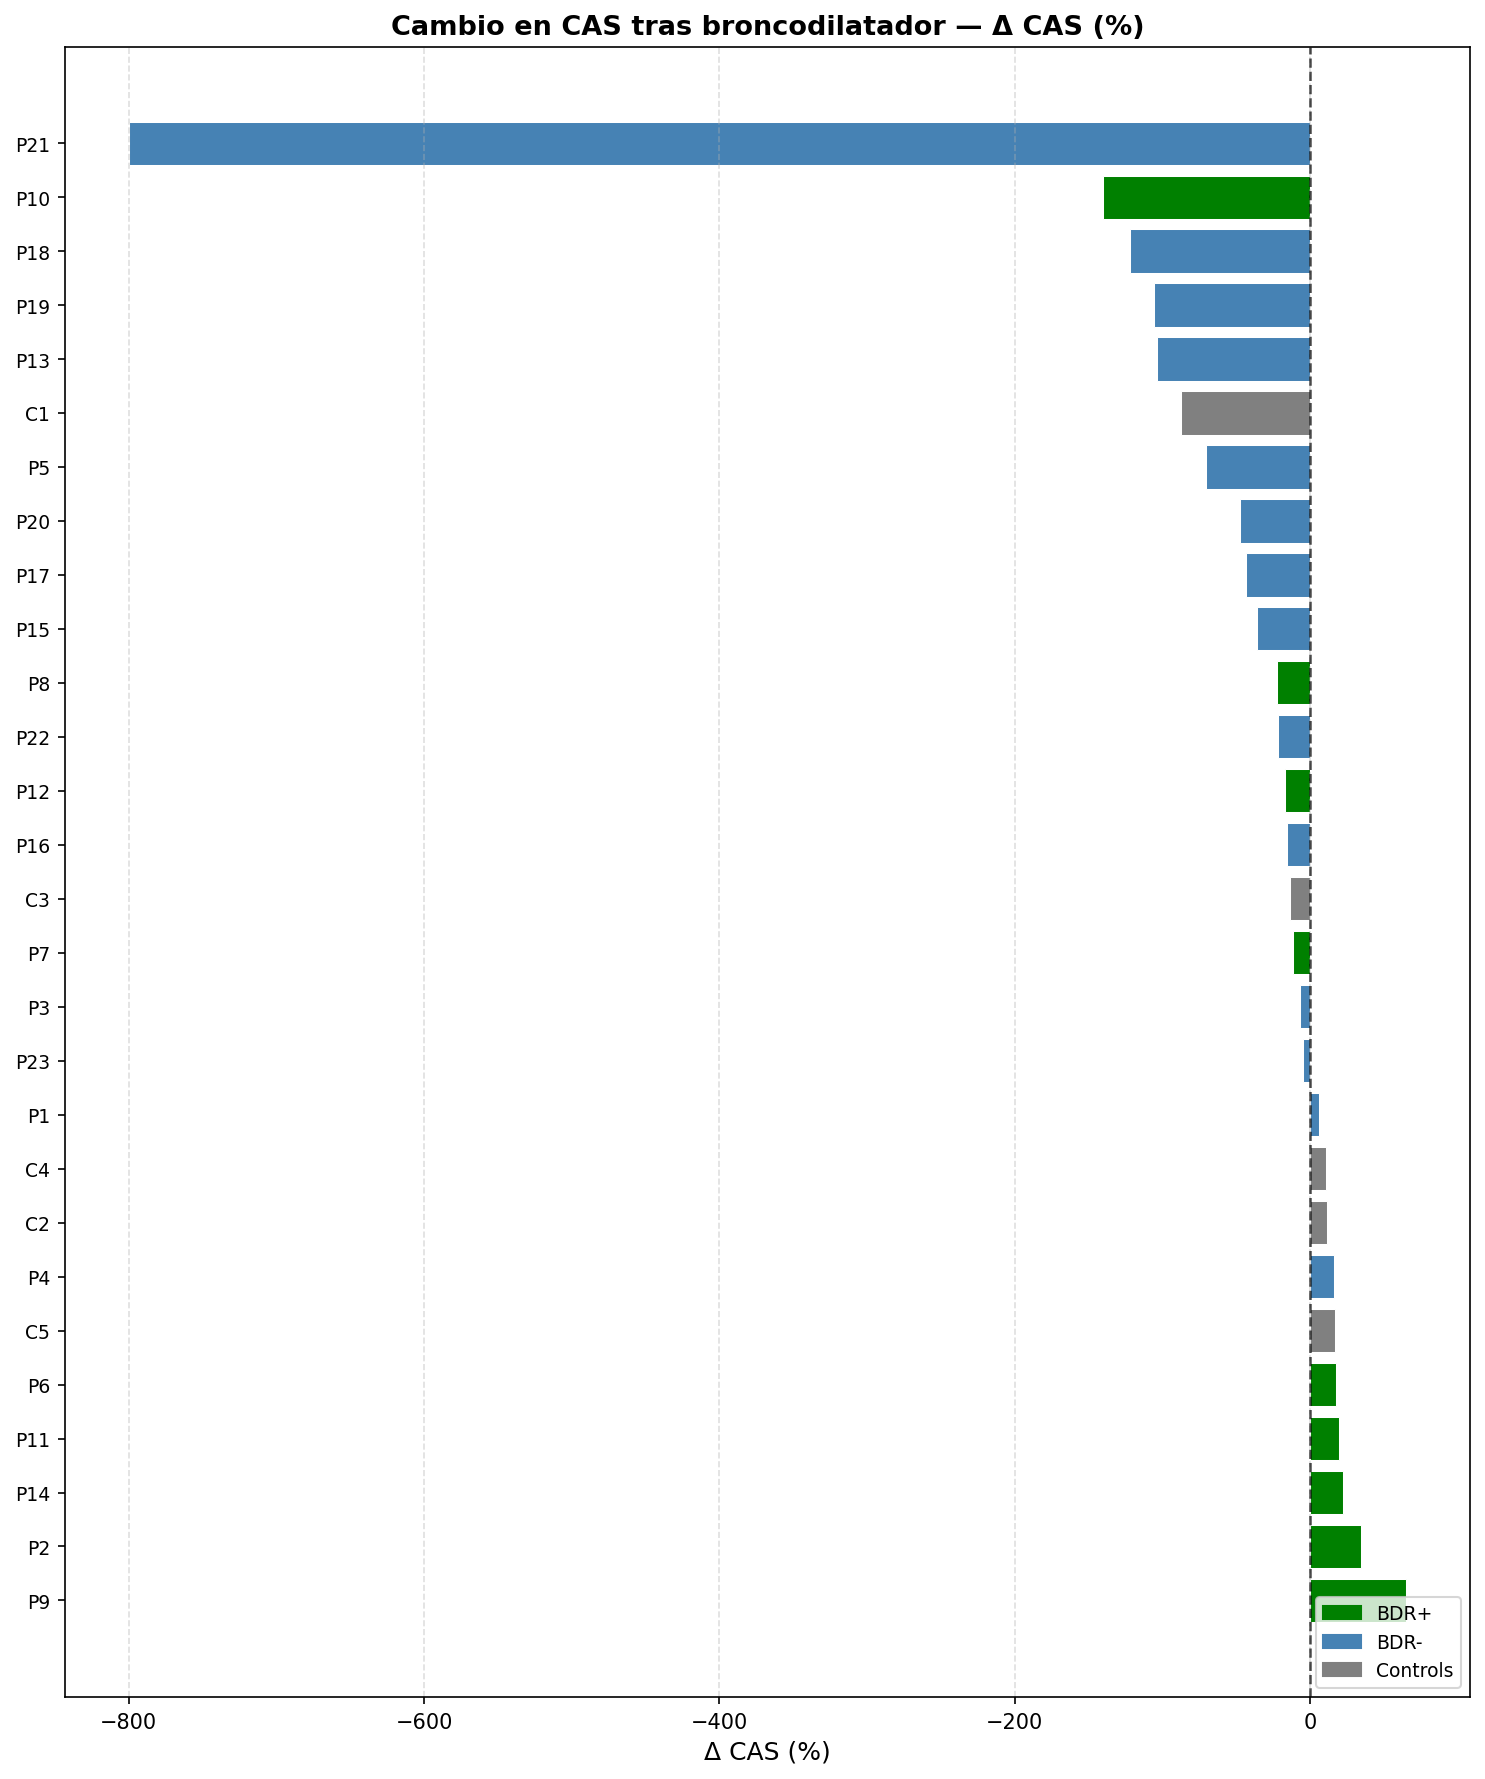
\includegraphics[width=0.80\linewidth]{fig2_delta_cas_per_subject.png}
  \end{block}
  {\small\textcolor{subtletext}{%
    Lorenzo Oliva \enspace\textperiodcentered\enspace
    Martina Vila López \enspace\textperiodcentered\enspace
    Adrià Font Plana \enspace\textperiodcentered\enspace
    Antoni Cardona Riera \enspace\textperiodcentered\enspace
    Gabriel Manzano Reche}}
\end{frame}

\end{document}

